\documentclass[conference]{IEEEtran}
\IEEEoverridecommandlockouts

\usepackage{amsmath,amssymb,amsfonts}
\usepackage{graphicx}
\usepackage{booktabs}
\usepackage{xcolor}
\usepackage{url}
\usepackage{microtype}

\graphicspath{{figures/}}

\begin{document}

\title{LCP-Nav: Latent Consequence Prediction for Cross-Domain Goal-Conditioned Visual Navigation}

\author{\IEEEauthorblockN{Author Name}
\IEEEauthorblockA{\textit{Department and Institution}\\
City, Country\\
author@email.com}}

\maketitle

\begin{abstract}
Goal-conditioned visual navigation supports mobile robots that traverse buildings, vegetation-rich paths, and campus roads. Yet route progress does not guarantee arrival: a direct policy may follow a route while stopping far from its visual goal because it does not evaluate alternative action consequences. We present Latent Consequence Prediction for Navigation (LCP-Nav), a lightweight policy that proposes finite trajectories, predicts their action-conditioned latent endpoints, and selects among them without generating future images. Five-seed cross-domain tests, matched diagnostics, and repeated Gazebo evaluations support improved transfer and closed-loop reliability while preserving real-time inference. These results motivate endpoint-aware navigation in campus-like environments, while claims remain limited to the evaluated datasets, checkpoint rules, and fixed simulation routes.
\end{abstract}

\begin{IEEEkeywords}
visual navigation, world models, latent dynamics, goal-conditioned navigation, mobile robots
\end{IEEEkeywords}

\section{Introduction}

Goal-conditioned visual navigation can support mobile robots moving between buildings, vegetation-rich paths, and campus roads from recent RGB observations and a goal image. Such routes amplify local errors: deviations can block constrained passages or accumulate into large terminal error. In our closed-loop audit, ViNT reaches 100\% mean campus progress but 0/5 validated arrivals and finishes $20.40\pm1.42$~m from the demonstration endpoint. Progress remains informative, but alone cannot certify arrival.

GNM and ViNT support transfer through shared action representations and heterogeneous robot data~\cite{gnm,vint}, yet directly predict local trajectories without comparing where alternatives may end. Pixel-generative world models provide such foresight by predicting future observations~\cite{nwm,uniwm}, but photorealistic generation is costly when used only for action ranking. Latent dynamics offer a lighter alternative if their representations remain non-degenerate. We therefore ask whether action-conditioned latent consequences can support endpoint-aware selection without changing the sensing interface.

LCP-Nav implements a propose--imagine--select pipeline: a deterministic head proposes $K$ trajectories, shared latent dynamics imagine their endpoints, and a scorer selects the endpoint most consistent with the goal. Future frames supervise only training, while SIGReg discourages latent collapse. Matched five-seed tests, functional interventions, and repeated simulation evaluate transfer, mechanism, arrival, and cost. The claim is bounded to a lightweight predictive bias under matched offline protocols and fixed campus-like Gazebo routes.

\section{Related Work}

\textbf{General visual-navigation policies.} ViNG introduced visual-goal navigation with topological memory~\cite{ving}; GNM standardized heterogeneous robot data~\cite{gnm}; and ViNT scaled a Transformer-based goal-conditioned policy~\cite{vint}. NoMaD added diffusion-based multimodal action generation and goal masking~\cite{nomad}. LiMo improves data efficiency by augmenting limited demonstrations with planner-generated supervision~\cite{limo}. Reports of zero-shot failures and collision-prone outputs show that direct RGB policies remain sensitive to domain and safety shifts~\cite{vfm-eval,care}. LCP-Nav addresses the narrower problem of comparing learned action consequences inside the policy and does not replace geometric safety systems.

\textbf{World models and latent prediction.} Navigation World Models generate action-conditioned future views for planning~\cite{nwm}, while UniWM couples visual foresight and action generation in an autoregressive model~\cite{uniwm}. ExploreVLA uses future RGB and depth generation as dense supervision for autonomous driving~\cite{explorevla}. LCP-Nav instead predicts latent endpoints and ranks a small deterministic candidate set, avoiding iterative sampling and pixel reconstruction. Its representation-learning motivation is related to LeWorldModel~\cite{lewm}, but the latent transition is trained jointly with distance estimation, trajectory generation, and candidate selection.

\begin{figure*}[t]
\centering
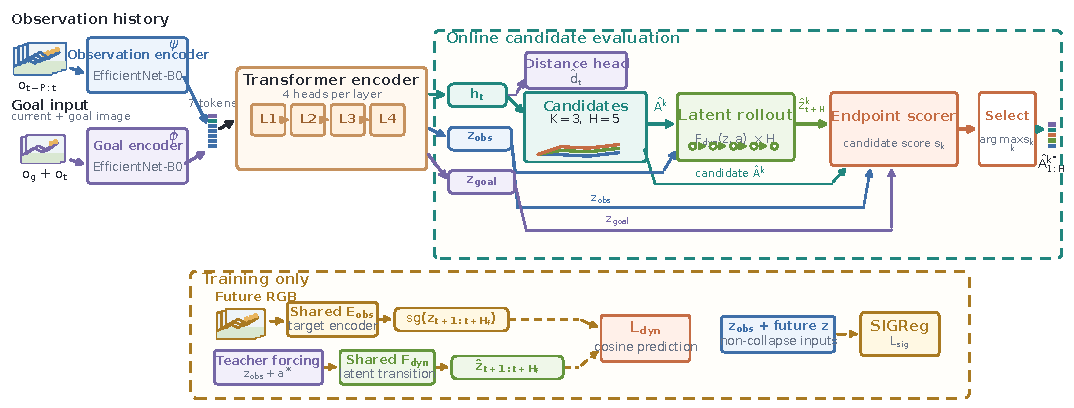
\includegraphics[width=0.99\textwidth]{fig1_lcp_architecture.pdf}
\caption{LCP-Nav architecture. The online path encodes the observation history and goal, predicts $K=3$ candidate trajectories, rolls each candidate through shared latent dynamics, and selects the highest-scoring imagined endpoint. Future images, expert-action teacher forcing, latent prediction loss, and SIGReg are used only during training.}
\label{fig:architecture}
\end{figure*}

\section{Method}

\subsection{Problem and Architecture}

Because route progress can remain high while terminal error grows, we formulate local planning as consequence-aware selection rather than single-trajectory regression. At time $t$, the policy receives $O_t=\{o_{t-P},\ldots,o_t\}$ and a goal image $o_g$. It predicts a temporal goal distance and an $H$-step local trajectory whose waypoint is $a_i=(\Delta x_i,\Delta y_i,\cos\theta_i,\sin\theta_i)$. Observation and goal encoders form tokens that a Transformer fuses into $h_t$. A candidate head then predicts
\begin{equation}
\{\hat A_t^1,\ldots,\hat A_t^K\}=f_{\mathrm{cand}}(h_t),
\end{equation}
where each candidate contains $H$ waypoints. Figure~\ref{fig:architecture} separates the deployed path from training-only supervision.


\subsection{Propose, Imagine, and Select}

LCP-Nav separates trajectory proposal from imagined-endpoint selection. For candidate $k$, the trajectory error combines mean Smooth-L1 position error and orientation cosine distance, $e_k=e_k^{\mathrm{pos}}+\lambda_\theta e_k^\theta$. Rather than hard best-of-$K$ assignment, candidate regression and ranking use soft targets
\begin{equation}
w_k=\frac{e^{-e_k/\tau_a}}{\sum_j e^{-e_j/\tau_a}},\qquad
q_k=\frac{e^{-e_k/\tau_s}}{\sum_j e^{-e_j/\tau_s}},
\end{equation}
with $L_{\mathrm{reg}}=\sum_k w_ke_k$ and $L_{\mathrm{score}}=-\sum_kq_k\log\operatorname{softmax}(s)_k$. The complete candidate objective is
\begin{equation}
L_{\mathrm{cand}}=L_{\mathrm{reg}}+L_{\mathrm{score}}+0.1L_{\mathrm{smooth}}+0.05L_{\mathrm{step}}+0.02L_{\mathrm{div}}.
\end{equation}
The smoothness and step terms suppress locally erratic motion, while $L_{\mathrm{div}}$ prevents all candidate endpoints from collapsing to the same location. We use $\lambda_\theta=1$, $\tau_a=\tau_s=1$, and a maximum single-step length of 1.5. The finite proposal has fixed cost and does not assume that the environment contains exactly $K$ action modes.

The shared transition predicts $\hat z_{t+1}=F_{\mathrm{dyn}}(z_t,a_t)$ and recursively rolls out each candidate,
\begin{equation}
\hat z_{t+h}^{k}=F_{\mathrm{dyn}}(\hat z_{t+h-1}^{k},\hat a_{t+h-1}^{k}).
\end{equation}
The scorer uses current, goal, endpoint, goal--endpoint difference, and encoded trajectory features to compute $s_k$; deployment selects $k^*=\arg\max_k s_k$. Thus, the model evaluates a predicted consequence rather than only regressing one trajectory from $h_t$.

The scorer receives $[z_t,z_g,\hat z_{t+H}^{k},z_g-\hat z_{t+H}^{k},\phi_A(\hat A^k)]$, where $\phi_A$ is a two-layer trajectory encoder. Candidate error provides the soft ranking target, avoiding geometric maps or endpoint-distance annotations. All candidates share transition parameters across rollout steps. Thus, increasing $K$ changes only the number of parallel rollouts, not the sensing interface.

\subsection{Predictive Training and Non-Collapse Regularization}

During training, expert actions drive a three-step teacher-forced rollout and real future frames provide stop-gradient targets. With validity mask $m_{b,h}$, the dynamics loss is
\begin{equation}
L_{\mathrm{dyn}}=\frac{\sum_{b,h}m_{b,h}[1-\cos(\hat z_{b,t+h},\operatorname{sg}(z_{b,t+h}))]}{\sum_{b,h}m_{b,h}}.
\end{equation}
Prediction alone can collapse distinct states. SIGReg instead matches one-dimensional random projections of observation and future tokens to a standard Gaussian. For embeddings $Z\in\mathbb{R}^{B\times T\times D}$, unit projections $r_m$, knots $u_l$, and $W=\sum_l\omega_l$, we compute
\begin{equation}
\begin{aligned}
L_{\mathrm{sig}}=\frac{1}{MW}\sum_{m,l}\omega_l\big[&\big(\mathbb{E}\cos(u_l Z^\top r_m)-e^{-u_l^2/2}\big)^2\\
&+\big(\mathbb{E}\sin(u_l Z^\top r_m)\big)^2\big].
\end{aligned}
\end{equation}
The expectation averages batch and temporal tokens. The complete objective is
\begin{equation}
L=L_{\mathrm{dist}}+L_{\mathrm{cand}}+\lambda_{\mathrm{dyn}}L_{\mathrm{dyn}}+\lambda_{\mathrm{sig}}L_{\mathrm{sig}}.
\end{equation}
The reported model uses $P=5$, $H=5$, $K=3$, 512-dimensional visual features, four Transformer layers, and $\lambda_{\mathrm{sig}}=0.12$. All online inputs are RGB images at $96\times96$; future images are absent at inference.

The supervised future-frame horizon is $H_f=3$, whereas deployment rolls each candidate through all $H=5$ action steps. The final two transitions are therefore short-horizon extrapolations. A validity mask removes unavailable future targets. SIGReg uses 1024 unit projections and 17 characteristic-function knots in $[0,3]$ without hard whitening. Training uses real future observations, but deployment requires only the observation history, goal image, and candidate actions.

\begin{figure*}[t]
\centering
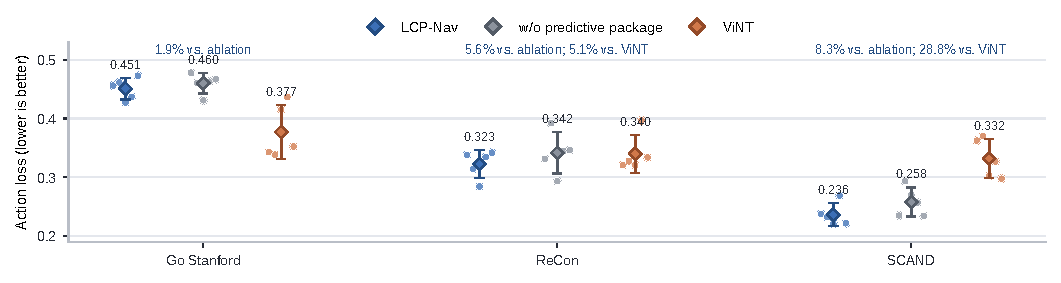
\includegraphics[width=0.98\textwidth]{fig2_offline_multiseed.pdf}
\caption{Five-seed offline action loss (points) with mean $\pm$ sample standard deviation (diamonds and bars). All checkpoints were selected on Go Stanford validation data; ReCon and SCAND are checkpoint-only zero-shot tests. The predictive-pathway ablation removes imagined endpoints, latent rollout, and dynamics supervision under otherwise matched training.}
\label{fig:offline}
\end{figure*}

\section{Experiments}

\subsection{Protocols}

\textbf{Offline evaluation.} Full LCP-Nav, a matched predictive-pathway ablation, and ViNT were trained independently with seeds 34, 38, 42, 43, and 44 on Go Stanford. The ablation preserves the inputs, backbone, action interface, data, and training budget. It removes imagined endpoints, action-conditioned rollout, and dynamics supervision. Validation action loss selects each checkpoint, which is then tested on fixed Go Stanford, ReCon, and SCAND samples. ReCon and SCAND use no fine-tuning or target-domain selection. Each complete seed-specific training run is one replicate ($n=5$).

All models use the runtime image size of $96\times96$, a six-frame observation sequence, and a five-waypoint action horizon. The visual encoder has dimension 512, the Transformer has four attention layers, and AdamW uses a learning rate of $8\times10^{-4}$. Data, optimization budget, validation protocol, and test samples are matched across the five-seed comparison. The evaluation manifest fixes sample indices, current and goal frames, negative-goal flags, and sampling seeds before paper-test reporting.

We predefine two checkpoint roles to prevent post hoc selection. LCP-Nav-action and ViNT are selected by validation action loss and used for all offline action comparisons. LCP-Nav-LFP is selected only by validation latent-prediction loss and is used for rollout diagnostics and closed-loop deployment. Paper-test, ReCon, SCAND, and Gazebo outcomes do not influence either selection rule. This separation avoids reporting the best checkpoint from multiple metrics after observing test performance.

Offline action loss averages Smooth-L1 waypoint-position error and orientation cosine distance over the five predicted waypoints. We additionally inspect waypoint cosine and orientation cosine to distinguish translation from heading quality. Cross-domain evaluation is checkpoint-only: every seed uses the Go Stanford validation-selected checkpoint without target-domain adaptation or reselection. Seed-level points, rather than frame-level samples, define uncertainty in Fig.~\ref{fig:offline}.

\textbf{Closed-loop evaluation.} Gazebo experiments use fixed indoor-obstacle, forest-road, and campus-road routes as controlled stress tests for constrained passage, appearance variation, and long-horizon terminal drift. Each method completes five runs per route, for 30 runs in total. Scene, route, poses, camera, chassis, controller, and topological procedure are held fixed. A validated arrival requires software-reported arrival, endpoint error no greater than 5~m, and no collision or timeout. LCP-Nav uses a validation latent-prediction checkpoint, whereas ViNT uses a validation action-loss checkpoint. The comparison therefore evaluates two predeclared deployment strategies rather than architecture alone.

Endpoint error is the Euclidean distance from the final robot position to the demonstration endpoint. Topological progress is the largest reached node index divided by the target-node index. Each replicate is a complete deployment of the same checkpoint. Closed-loop outcomes are never used for checkpoint selection.

During deployment, LCP-Nav generates three local trajectories in one forward pass, rolls each through the shared dynamics model, and executes the highest-scoring candidate. ViNT executes its direct trajectory output. Both policies use the same camera stream, chassis limits, control frequency, topological graph, and arrival detector. The five repetitions per scene begin from matched poses and headings. Runs terminate only through reported arrival, collision, timeout, or the fixed route procedure, so failed trajectories are not truncated for analysis.


\begin{figure*}[t]
\centering
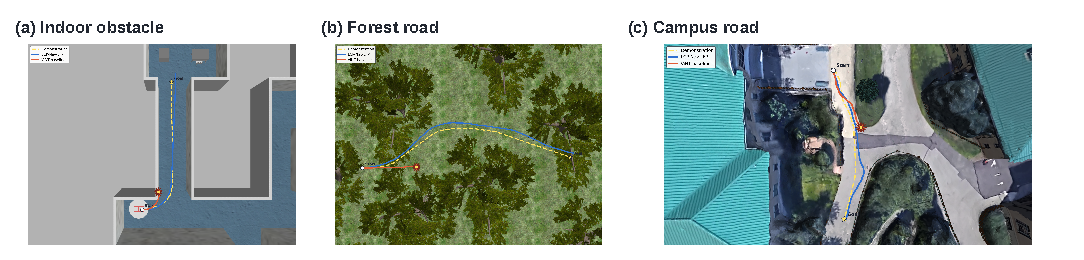
\includegraphics[width=0.96\textwidth]{fig3_overhead_scene_context.pdf}
\vspace{0.35em}
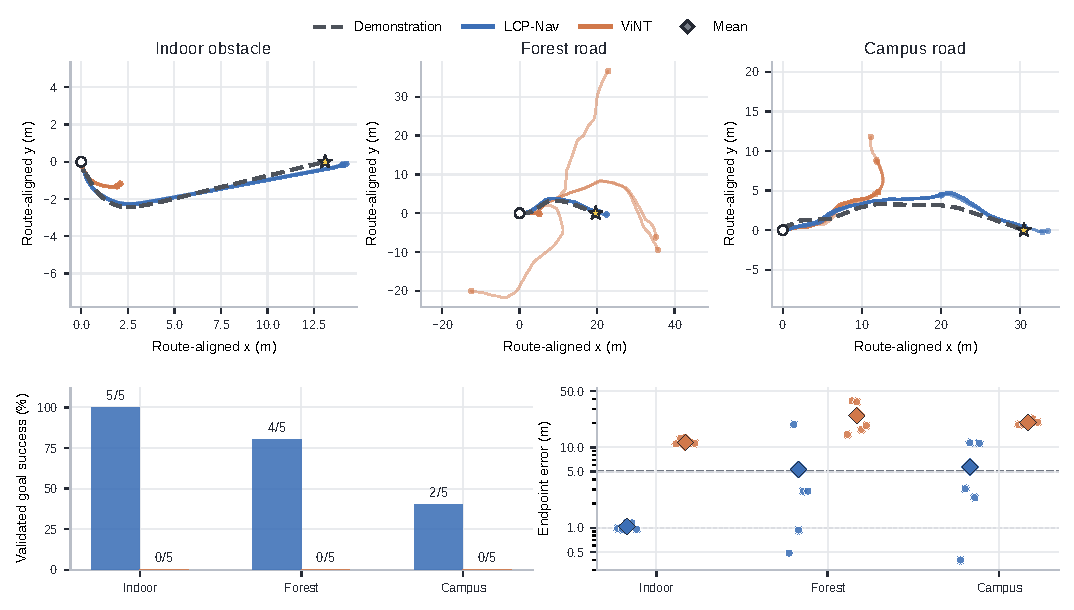
\includegraphics[width=0.96\textwidth,trim=0 0 0 175bp,clip]{fig3_closed_loop_simulation.pdf}
\caption{Scenario-driven closed-loop Gazebo evaluation. The routes stress constrained passage, appearance variation, and terminal drift. Top: calibrated overhead views; the dashed yellow line is the demonstration route, blue and orange are retained LCP-Nav and ViNT trajectories, circles mark starts, stars mark demonstration endpoints, and burst symbols mark failure stops. Bottom: validated arrivals and endpoint error for all five runs per method and scene (diamonds denote means; endpoint error uses a log scale; dashed lines mark 1 and 5~m).}
\label{fig:simulation}
\end{figure*}

\subsection{Does Consequence Prediction Improve Transfer?}

To test whether the predictive pathway improves transfer under matched training, Fig.~\ref{fig:offline} reports all five seed-level action losses. LCP-Nav reduces mean loss relative to the matched ablation from 0.4599 to 0.4510 on Go Stanford, 0.3416 to 0.3226 on ReCon, and 0.2579 to 0.2363 on SCAND. The corresponding reductions are 1.9\%, 5.6\%, and 8.3\%. ViNT remains stronger in-domain (0.3771), but LCP-Nav is lower on ReCon (0.3226 versus 0.3399) and SCAND (0.2363 versus 0.3319). All five SCAND seeds improve over ViNT, with a paired mean difference of $-0.0955$ and a 95\% exhaustive-bootstrap interval of $[-0.1228,-0.0698]$. The increasing gain over the matched ablation links transfer improvement more directly to the predictive pathway.

Cross-domain values were also audited in physical units. Go Stanford, ReCon, and SCAND use waypoint spacings of 0.12, 0.25, and 0.38~m, respectively. Recomputing translation and orientation metrics with these scales preserves the reported transfer pattern, so the gain is not produced by one normalization convention. Split audits found no trajectory intersections between training and test sets in any domain and no overlap between Go Stanford validation and test trajectories.


We next test whether the learned pathway performs the intended decision role. At $\lambda_{\mathrm{sig}}=0.12$, $K=3$ yields lower action loss (0.3919) than $K=1$ (0.4318) or $K=5$ (0.4685). Without SIGReg, the best latent-prediction loss falls to 0.0023, but effective rank collapses to 1.02 and the first eigenvalue explains 99.7\% of variance. Cyclically permuting only the imagined endpoint reduces candidate-selection agreement by about 43\% across all datasets. The scorer therefore uses endpoint features rather than treating them as redundant inputs. These single-run diagnostics explain the selected design but do not carry the main statistical claim.

Multi-seed rollouts test whether the transition remains useful recursively. For action-selected checkpoints, one-, two-, and three-step latent MSEs are 1.653, 2.318, and 2.732. The matched ablation gives 3.743, 4.195, and 4.604, corresponding to reductions of 55.8\%, 44.7\%, and 40.7\%. Predictive checkpoints retain third-step cosine consistency of $0.9024\pm0.0387$, whereas the ablation falls to $0.5098\pm0.0529$. In the paired intervention, candidate trajectories and current/goal latents remain fixed while endpoint features are permuted. Agreement decreases by 43.6\%, 42.7\%, and 43.2\% on Go Stanford, ReCon, and SCAND. These tests connect latent prediction to the deployed decision chain.

\subsection{Does Route Progress Translate into Arrival?}

To test whether the predictive pathway changes endpoint reliability, Fig.~\ref{fig:simulation} combines spatial context with repeated-run evidence. The overhead panels retain scene geometry, the demonstration route, and one raw trajectory from each method. The lower panels report all five runs per method and scene.


The overhead panels locate obstacle-passage failures indoors, route deviation in the forest, and terminal-position error on campus. They provide qualitative context, while the lower panels summarize every recorded run.

The lower panels report the primary deployment outcomes. LCP-Nav obtains 5/5, 4/5, and 2/5 validated arrivals indoors, in the forest, and on campus; ViNT obtains 0/5 throughout. Totals are 11/15 (73.3\%) and 0/15. Mean endpoint errors are 1.036, 5.299, and 5.697~m for LCP-Nav, compared with 11.563, 24.914, and 20.404~m for ViNT. On campus, ViNT reaches 100\% mean node progress but remains about 20~m from the endpoint. Thus, topological progress alone does not establish arrival.

\begin{table}[t]
\centering
\caption{Repeated closed-loop simulation (mean $\pm$ sample standard deviation; $n=5$ runs per method and scene).}
\label{tab:closedloop}
\setlength{\tabcolsep}{3.2pt}
\footnotesize
\begin{tabular}{@{}llccc@{}}
\toprule
Scene & Method & Arrival & Error (m) & Progress (\%) \\
\midrule
Indoor & LCP-Nav & 5/5 & $1.04\pm0.10$ & $100.0\pm0.0$ \\
       & ViNT    & 0/5 & $11.56\pm0.83$ & $48.2\pm27.3$ \\
Forest & LCP-Nav & 4/5 & $5.30\pm7.93$ & $79.2\pm42.1$ \\
       & ViNT    & 0/5 & $24.91\pm11.43$ & $44.8\pm11.4$ \\
Campus & LCP-Nav & 2/5 & $5.70\pm5.24$ & $83.8\pm17.5$ \\
       & ViNT    & 0/5 & $20.40\pm1.42$ & $100.0\pm0.0$ \\
\bottomrule
\end{tabular}
\end{table}


Scene-wise variation clarifies the aggregate count. Indoors, LCP-Nav succeeds in every run with only $0.10$~m standard deviation in endpoint error. ViNT reaches $48.2\%\pm27.3\%$ mean progress and stops far from the endpoint. In the forest, one failure raises LCP-Nav error to $5.30\pm7.93$~m despite four arrivals. On campus, LCP-Nav reaches $83.8\%\pm17.5\%$ progress but validates only two arrivals, revealing residual long-horizon drift. ViNT records full node progress yet finishes at $20.40\pm1.42$~m error. The composite criterion therefore distinguishes route traversal from accurate termination.

A stricter 1-m endpoint threshold, combined with software-reported arrival and no collision or timeout, accepts 6/15 LCP-Nav runs and 0/15 ViNT runs. This sensitivity check shows that the 5-m result is not solely an artifact of a permissive radius. Complete runs remain the experimental unit, and failures remain in the endpoint-error distribution in Fig.~\ref{fig:simulation}.


Policy-only efficiency was measured after 100 warm-up iterations and over 500 repetitions using inputs $\mathrm{obs}=[1,6,3,96,96]$ and $\mathrm{goal}=[1,3,96,96]$. LCP-Nav contains 26.77~M parameters, 9.8\% fewer than ViNT at 29.66~M, and requires approximately 1.164~GFLOPs. On an RTX~4090 with float32 inputs, p95 latency is 24.3--24.8~ms, compared with 22.6~ms for ViNT. Peak allocated memory is 129.6--131.3~MiB, below the ViNT value of 142.7~MiB. Finite latent rollouts therefore preserve policy inference above 40~Hz with a small measured latency increment.

\section{Discussion}

The central finding is that route progress and terminal arrival are not interchangeable in the evaluated campus-like routes. ViNT's full mean campus progress but large endpoint error exposes this gap. LCP-Nav addresses it by separating trajectory proposal from consequence-aware selection. Transfer, rollout, endpoint-intervention, and closed-loop results support this role at real-time speed.

The three routes approximate constrained passage, vegetation-rich appearance variation, and terminal drift between campus buildings, green paths, and roads, but do not constitute physical-campus validation or a safety system. Different checkpoint objectives make the closed-loop comparison one between predeclared deployment strategies; five repetitions estimate fixed-route stability only; and validated arrival is not a formal safety guarantee. Physical tests should use matched checkpoints, additional routes, illumination changes, pedestrians, and dynamic obstacles while retaining endpoint error and failure cause.

\section{Conclusion}

LCP-Nav makes goal-conditioned navigation endpoint-aware by combining finite proposals, latent rollout, imagined-endpoint selection, and non-collapse regularization. Five-seed tests and repeated Gazebo runs support improved transfer and endpoint reliability within a real-time budget. The evidence remains bounded to the present datasets and fixed simulations, motivating matched-checkpoint tests on physical campus routes.

\begin{thebibliography}{00}
\bibitem{ving} D. Shah, B. Eysenbach, G. Kahn, N. Rhinehart, and S. Levine, ``ViNG: Learning open-world navigation with visual goals,'' in \emph{Proc. IEEE Int. Conf. Robot. Autom.}, 2021.
\bibitem{gnm} D. Shah, A. Sridhar, A. Bhorkar, N. Hirose, and S. Levine, ``GNM: A general navigation model to drive any robot,'' in \emph{Proc. IEEE Int. Conf. Robot. Autom.}, 2023.
\bibitem{vint} D. Shah \emph{et al.}, ``ViNT: A foundation model for visual navigation,'' in \emph{Proc. Conf. Robot Learn.}, vol. 229, pp. 711--733, 2023.
\bibitem{nomad} A. Sridhar, D. Shah, C. Glossop, and S. Levine, ``NoMaD: Goal masked diffusion policies for navigation and exploration,'' arXiv:2310.07896, 2023.
\bibitem{vfm-eval} M. Guerrier, K. Soma, J. Pavlasek, and G. Beltrame, ``Can vision foundation models navigate? Zero-shot real-world evaluation and lessons learned,'' arXiv:2603.25937, 2026.
\bibitem{care} J. Kim, J. Sim, W. Kim, K. Sycara, and C. Nam, ``CARE: Enhancing safety of visual navigation through collision avoidance via repulsive estimation,'' in \emph{Proc. 9th Conf. Robot Learn.}, 2025.
\bibitem{limo} Y. Inglin, J. Frey, C. Chen, and M. Hutter, ``Less is more: Scalable visual navigation from limited data,'' arXiv:2601.17815, 2026.
\bibitem{nwm} A. Bar, G. Zhou, D. Tran, T. Darrell, and Y. LeCun, ``Navigation world models,'' arXiv:2412.03572, 2024.
\bibitem{uniwm} Y. Dong \emph{et al.}, ``Unified world models: Memory-augmented planning and foresight for visual navigation,'' arXiv:2510.08713, 2025.
\bibitem{explorevla} Z. Sheng, X. Ye, J. Luo, S. Chen, and L. Ren, ``ExploreVLA: Dense world modeling and exploration for end-to-end autonomous driving,'' arXiv:2604.02714, 2026.
\bibitem{lewm} L. Maes, Q. Le Lidec, D. Scieur, Y. LeCun, and R. Balestriero, ``LeWorldModel: Stable end-to-end joint-embedding predictive architecture from pixels,'' arXiv:2603.19312, 2026.
\end{thebibliography}

\end{document}
